\section{Meta Model}\label{metamodel}
The classes in the Ecore meta-model are described in this section along
with the OCLinEcore validation steps that are applied.

For reference, the full meta-model is displayed first and the individual
components after.
\begin{figure}[ph]
    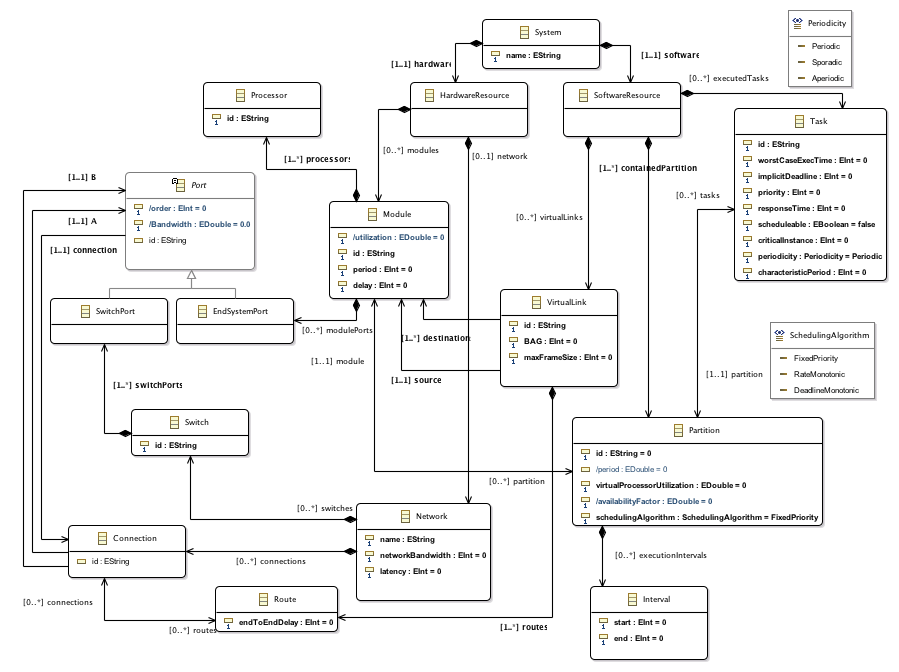
\includegraphics[width=\textwidth]{metamodel_full.png}
    \caption{Full UML meta-model}
    \label{fig:fullmodel} % adding labels for references
\end{figure}

% Now all of the model elements
\begin{description}
    \item[System] \hfill \\
        The root object for an instance of the meta model. \\
        \textbf{Constraints} 
\end{description}
